\subsection{Manipulasi Informasi pada Gerbang 2 \textit{Qubit}}
Keterbelitan kuantum atau \textit{entanglement} merupakan fenomena non-lokal di mana keadaan satu \textit{qubit} tidak dapat didefinisikan secara independen dari keadaan \textit{qubit} lainnya dalam sistem multikomponen. Sebelum memahami keterbelitan pada sistem yang kompleks, perlu dipahami konsep Keadaan Bell (\textit{Bell States}) yang merupakan representasi dari keterbelitan maksimal antara dua \textit{qubit} terisolasi. Terdapat empat jenis Keadaan Bell yang membentuk basis ortonormal bagi ruang Hilbert dua-\textit{qubit} untuk merangkum seluruh probabilitas korelasi sistem fisis:
\begin{equation}
\label{eq:bell_states}
    |\Phi^{\pm}\rangle = \frac{|00\rangle \pm |11\rangle}{\sqrt{2}}, \quad |\Psi^{\pm}\rangle = \frac{|01\rangle \pm |10\rangle}{\sqrt{2}}.
\end{equation}
Keadaan Bell menunjukkan korelasi non-klasik yang sangat kuat, di mana tindakan pengukuran pada satu \textit{qubit} akan secara instan menentukan status keadaan \textit{qubit} lainnya meskipun keduanya terpisah secara fisik.

Pembangkitan keadaan Bell tersebut secara teknis dapat direkonstruksi dari basis komputasi dua \textit{qubit} melalui kombinasi linear gerbang Hadamard satu \textit{qubit} dengan gerbang dua \textit{qubit} \textit{Controlled-NOT} (CNOT)~\cite{mitarai_quantum_2018,innan_quantum_2025}. Secara matematis, langkah awal dilakukan dengan menerapkan transformasi gerbang Hadamard pada \textit{qubit} pertama yang diikuti dengan operasi identitas pada \textit{qubit} kedua:
\begin{equation}
(H\otimes I)|00\rangle = \frac{|00\rangle + |10\rangle}{\sqrt{2}}.
\end{equation}
Setelah itu, penerapan \textit{operator} CNOT pada keadaan superposisi tersebut memicu efek keterbelitan maksimal yang menghasilkan keadaan Bell pertama secara presisi:
\begin{equation}
\text{CNOT}\left(\frac{|00\rangle + |10\rangle}{\sqrt{2}}\right) = \frac{|00\rangle + |11\rangle}{\sqrt{2}} = |\Phi^+\rangle.
\end{equation}

Bentuk umum pemetaan dari seluruh basis komputasi dua \textit{qubit} menuju himpunan basis keadaan Bell tersebut dapat dituliskan secara komprehensif melalui relasi persamaan \textit{uniter} berikut:
\begin{equation}
\label{eq:bell_transformations}
\begin{split}
|\Phi^+\rangle &= \text{CNOT}(H\otimes I)|00\rangle, \quad |\Psi^+\rangle = \text{CNOT}(H\otimes I)|01\rangle, \\
|\Phi^-\rangle &= \text{CNOT}(H\otimes I)|10\rangle, \quad |\Psi^-\rangle = \text{CNOT}(H\otimes I)|11\rangle.
\end{split}
\end{equation}
Persamaan pemetaan uniter tersebut membuktikan bahwa \textit{operator} transformasi gabungan $U_{\text{Bell}} = \text{CNOT}(H\otimes I)$ secara fisis memetakan basis komputasi menuju basis Bell terbelit secara sempurna. Melalui formulasi perkalian luar (\textit{outer product}), representasi \textit{operator} transformasi basis kuantum tersebut dapat dituliskan secara rinci sebagai jumlahan proyeksi keadaan sebagai berikut:
\begin{equation}
\label{eq:u_bell_outer}
U_{\text{Bell}} = |\Phi^+\rangle\langle 00| + |\Psi^+\rangle\langle 01| + |\Phi^-\rangle\langle 10| + |\Psi^-\rangle\langle 11|.
\end{equation}

Untuk mendapatkan \textit{operator} CNOT dari representasi basis Bell, persamaan gabungan tersebut dikalikan dengan \textit{operator} invers dari transformasi Hadamard dari arah kanan. Karena \textit{operator} Hadamard bersifat \textit{self-inverse} yang berarti memiliki nilai invers sama dengan \textit{matriks} asalnya, maka \textit{operator} CNOT dapat ditransformasikan secara aljabar:
\begin{equation}
\label{eq:cnot_from_bell}
\text{CNOT} = U_{\text{Bell}}(H\otimes I) = \Big( |\Phi^+\rangle\langle 00| + |\Psi^+\rangle\langle 01| + |\Phi^-\rangle\langle 10| + |\Psi^-\rangle\langle 11| \Big) (H\otimes I).
\end{equation}
Persamaan di atas menunjukkan bahwa \textit{operator} CNOT dapat dibangun sepenuhnya dari deskripsi keadaan Bell dan transformasi Hadamard pada sistem kuantum. Dengan memasukkan definisi dari masing-masing keadaan Bell pada persamaan (\ref{eq:bell_states}) ke dalam perkalian luar tersebut, diperoleh representasi \textit{matriks} \textit{operator} \textit{uniter} yang mewakili gerbang tersebut.

Sebagai alternatif konstruksi langsung tanpa melibatkan gerbang Hadamard, \textit{operator} CNOT juga dapat didefinisikan secara langsung melalui aksi pemetaan basis komputasi~\cite{peruzzo_variational_2014}. Aksi pemetaan tersebut membalikkan status keadaan \textit{qubit} target apabila status keadaan \textit{qubit} kontrol bernilai satu, yang secara aljabar dituliskan sebagai:
\begin{equation}
\label{eq:cnot_actions}
\text{CNOT}|00\rangle = |00\rangle, \quad \text{CNOT}|01\rangle = |01\rangle, \quad \text{CNOT}|10\rangle = |11\rangle, \quad \text{CNOT}|11\rangle = |10\rangle.
\end{equation}
Dengan menggunakan aksi pemetaan basis komputasi tersebut, formulasi perkalian luar dari \textit{operator} CNOT dapat didefinisikan secara langsung melalui relasi jumlahan proyeksi keadaan:
\begin{equation}
\label{eq:cnot_outer_direct}
\text{CNOT} = |00\rangle\langle 00| + |01\rangle\langle 01| + |11\rangle\langle 10| + |10\rangle\langle 11|.
\end{equation}
Melalui evaluasi bentuk perkalian luar tersebut pada basis komputasi dua \textit{qubit}, \textit{matriks} \textit{uniter} dari gerbang CNOT dapat diturunkan secara eksplisit sesuai dengan arah kontrolnya:
\begin{equation}
\label{eq:cnot_matrices}
\text{CNOT}_{01} = \begin{pmatrix} 1 & 0 & 0 & 0 \\ 0 & 1 & 0 & 0 \\ 0 & 0 & 0 & 1 \\ 0 & 0 & 1 & 0 \end{pmatrix}, \quad \text{CNOT}_{10} = \begin{pmatrix} 1 & 0 & 0 & 0 \\ 0 & 0 & 0 & 1 \\ 0 & 0 & 1 & 0 \\ 0 & 1 & 0 & 0 \end{pmatrix}.
\end{equation}

Dalam konteks optimasi portofolio finansial, fenomena \textit{entanglement} dimanfaatkan secara cerdas untuk merepresentasikan hubungan ketergantungan dan \textit{matriks} korelasi silang antar berbagai variabel aset ekonomi secara efisien. Representasi visual dari mekanisme operasional gerbang CNOT diilustrasikan pada Gambar \ref{fig:gerbang_cnot}, yang secara rinci menunjukkan interaksi antara \textit{qubit} kontrol dengan titik hitam ($\bullet$) dan \textit{qubit} target dengan simbol plus dilingkari ($\oplus$).
\begin{figure}[htbp]
    \centering
    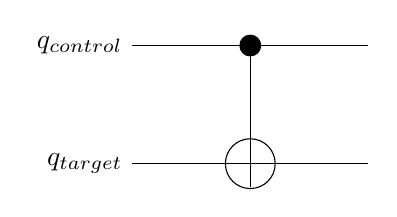
\begin{tikzpicture}[scale=1.5, >=stealth]
        \draw (0,1.5) -- (2,1.5) node[pos=0, left] {$q_{control}$};
        \draw (0,0.5) -- (2,0.5) node[pos=0, left] {$q_{target}$};
        \filldraw (1,1.5) circle (2.5pt);
        \draw (1,1.5) -- (1,0.5);
        \draw (1,0.5) circle (6pt);
        \draw (1,0.3) -- (1,0.7);
        \draw (0.8,0.5) -- (1.2,0.5);
    \end{tikzpicture}
    \caption{Representasi simbolik gerbang keterbelitan (\textit{Controlled-NOT}) yang mengilustrasikan interaksi non-lokal antar \textit{qubit} dalam sistem sirkuit.}
    \label{fig:gerbang_cnot}
\end{figure}

\subsection{Sirkuit Kuantum Berparameter}
\textit{Quantum Machine Learning} (QML) merupakan bidang multidisipliner yang menggabungkan prinsip komputasi kuantum dengan metode pemelajaran mesin. Salah satu pendekatan yang berkembang dalam QML adalah \textit{Quantum Deep Learning} (QDL), yaitu pemanfaatan model kuantum dengan parameter khusus untuk mempelajari pemodelan data kompleks. Implementasi model QDL umumnya diwujudkan melalui \textit{Parameterized Quantum Circuit} (PQC), yaitu sirkuit kuantum yang terdiri atas gerbang-gerbang kuantum yang memiliki parameter yang nilainya dapat dioptimasi. PQC menjadi komponen utama dalam keluarga \textit{Variational Quantum Algorithms} (VQA), yaitu algoritma hibrida yang menggabungkan pemrosesan kuantum dan optimasi klasik. Keluarga VQA terdiri dari \textit{Variational Quantum Eigensolver} (VQE), \textit{Quantum Approximate Optimization Algorithm} (QAOA), dan Variational Quantum Classifier (VQC) yang mana semuanya memanfaatkan PQC sebagai representasi solusi yang dievaluasi untuk kemudian nilainya diperbarui oleh algoritma optimasi klasik secara iteratif~\cite{reifenstein_coherent_2021,anshu_sample-efficient_2020,chen_enhanced_2025}.

Sirkuit Kuantum Berparameter (\textit{Parameterized Quantum Circuit} atau PQC) adalah rangkaian gerbang kuantum yang memiliki parameter kontinu, umumnya berupa sudut rotasi. Dalam algoritma variasional, rangkaian PQC berperan sebagai ansatz yang mengeksplorasi parameter pada ruang solusi untuk fungsi gelombang dari suatu permasalahan. Pada umumnya, alur kerja PQC ditunjukkan pada Gambar \ref{fig:pqc_workflow}. Secara singkat, proses diawali dengan penyandian data klasik $x \in \mathbb{R}^n$ ke dalam keadaan kuantum $|\psi_0\rangle$ melalui fungsi prapemrosesan $f(x)$ dan operasi penyandian $R(f(x))$. Keadaan kuantum yang telah terbentuk kemudian diproses oleh sirkuit variasional $U(\boldsymbol{\theta})$, yang bertugas mentransformasikan keadaan kuantum melalui serangkaian operasi kuantum berparameter. Parameter $\boldsymbol{\theta}$ pada sirkuit ini akan diperbarui secara iteratif selama proses optimasi untuk menghasilkan suatu keadaan kuantum $|\psi(\boldsymbol{\theta})\rangle$ yang merepresentasikan solusi optimum. Selanjutnya, keadaan akhir diproyeksikan melalui pengukuran $\{M\}$ untuk memperoleh nilai ekspektasi atau probabilitas observabel yang relevan. Hasil pengukuran tersebut kemudian dievaluasi menggunakan fungsi biaya $L(\boldsymbol{\theta})$, yang digunakan oleh algoritma optimasi klasik untuk menentukan pembaruan parameter hingga diperoleh parameter optimal $\boldsymbol{\theta}^∗$ dan keluaran model $y \in \mathbb{R}^n$.
\begin{figure}[htbp]
    \centering
    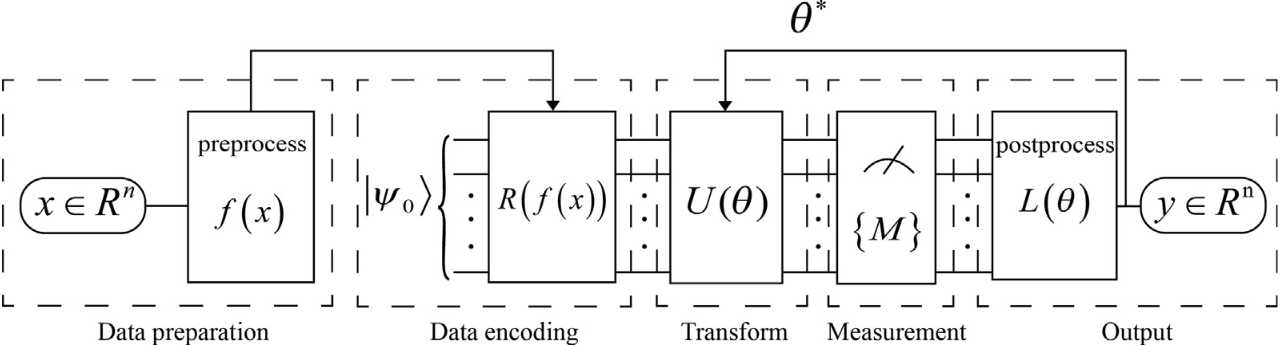
\includegraphics[width=0.7\textwidth]{Images/PQC_VQDNN.png}
    \caption[Representasi alur kerja sirkuit kuantum berparameter (PQC) yang mengilustrasikan tahap penyandian data, sirkuit variasional, pengukuran, dan pembaruan parameter oleh algoritma optimasi klasik \cite{regadio_exoplanet_2025}
    \label{fig:pqc_workflow}
\end{figure}

Setelah data dikodekan ke dalam keadaan kuantum $|\psi(\boldsymbol{\theta})\rangle$, sirkuit variasional $U(\boldsymbol{\theta})$ diterapkan untuk menghasilkan keadaan kuantum yang bergantung pada parameter-parameter optimasi. Berdasarkan sifat evolusi uniter dalam mekanika kuantum, keadaan keluaran sirkuit dapat dituliskan sebagai
\begin{equation}
\label{eq:vqa_state}
|\psi(\boldsymbol{\theta})\rangle = U(\boldsymbol{\theta})|\psi_0\rangle.
\end{equation}
di mana operator variasional $U(\boldsymbol{\theta})$ dibangun dari kombinasi gerbang rotasi satu-qubit dan gerbang keterbelitan dua-qubit. Secara umum, operator tersebut dapat dinyatakan
\begin{equation}
    U(\boldsymbol{\theta}) = \prod_{l=1}^L U_{(ent)}^{(l)} U_{(rot)}^{(l)} (\boldsymbol{\theta}^{(l)})
\end{equation}
dengan $U_{(rot)}^{(l)}$ merepresentasikan lapisan gerbang rotasi berparameter, seperti $Rx(\theta)$, $Ry(\theta)$, dan $Rz (\theta)$, sedangkan $U_{(ent)}^{(l)}$ menyatakan lapisan gerbang keterbelitan, misalnya gerbang CNOT. Struktur berlapis ini memungkinkan sirkuit menghasilkan keadaan kuantum yang semakin kompleks seiring bertambahnya jumlah parameter dan lapisan yang digunakan. Variasi nilai parameter $\boldsymbol{\theta}$ akan menghasilkan fungsi gelombang yang berbeda sehingga memungkinkan eksplorasi berbagai kandidat solusi di dalam ruang pencarian.

Kualitas suatu kandidat solusi kemudian dievaluasi melalui pengukuran nilai ekspektasi suatu operator observabel $\hat{O}$, yang umumnya merepresentasikan fungsi biaya atau besaran fisik yang ingin dioptimalkan. Nilai fungsi biaya tersebut dirumuskan sebagai
\begin{equation}
\label{eq:vqa_cost}
C(\boldsymbol{\theta}) = \langle \psi(\boldsymbol{\theta})| \hat{O} |\psi(\boldsymbol{\theta})\rangle.
\end{equation}
Nilai hasil pengukuran tersebut kemudian dikirimkan kepada \textit{optimizer} klasik untuk memperbarui parameter sirkuit, kemudian proses evaluasi dan pembaruan diulang hingga kriteria konvergensi terpenuhi. Proses ini dikenal sebagai \textit{hybrid quantum-classical optimization} atau optimasi hibrida kuantum-klasik.


\subsection{Pengukuran Kuantum}
Pengukuran merupakan tahap yang menghubungkan informasi kuantum dengan hasil observasi klasik yang dapat diakses oleh pengguna. Dalam mekanika kuantum, setiap besaran fisik direpresentasikan oleh suatu operator observabel Hermitian $\hat{O}$ yang memiliki himpunan nilai eigen $o_n$ dan vektor eigen ortonormal $|e_n\rangle$. Hubungan antara observabel dan basis eigennya dinyatakan melalui persamaan
\begin{equation}
\hat{O}|e_n\rangle = o_n |e_n\rangle.
\end{equation}
Jika suatu sistem berada pada keadaan $|\psi\rangle$, maka hasil pengukuran yang mungkin diperoleh hanyalah nilai-nilai eigen dari operator observabel tersebut. Untuk sebuah qubit yang berada pada keadaan superposisi
\begin{equation}
|\psi\rangle = a|0\rangle + b|1\rangle,
\end{equation}
probabilitas diperolehnya suatu hasil pengukuran ditentukan oleh kaidah Born (\textit{Born rule}). tersebut menyatakan bahwa probabilitas untuk memperoleh nilai eigen $o_n$ diberikan oleh proyeksi keadaan terhadap basis eigen observabel,
\begin{equation}
P(o_n) = |\langle e_n|\psi\rangle|^2.
\end{equation}
Sehingga, pada basis komputasi, probabilitas diperolehnya keadaan $|0\rangle$ dan $|1\rangle$ menjadi
\begin{equation} P(0)=|a|^2, \qquad P(1)=|b|^2.
\end{equation}
Hal tersebut menginterpretasi probabilistik ini menunjukkan bahwa hasil pengukuran tidak dapat diprediksi secara deterministik untuk satu percobaan tunggal, melainkan hanya dapat diprediksi melalui distribusi probabilitas hasil pengukuran.

Secara matematis, proses pengukuran direpresentasikan menggunakan operator proyeksi
\begin{equation} \hat{P}_n = |e_n\rangle\langle e_n|.
\end{equation}
Jika hasil pengukuran yang diperoleh adalah nilai eigen $o_n$, maka keadaan sistem setelah pengukuran diberikan oleh
\begin{equation}
|\psi'\rangle = \frac{\hat{P}_n|\psi\rangle} {\sqrt{\langle\psi|\hat{P}_n|\psi\rangle}}.
\end{equation}
Persamaan tersebut menunjukkan bahwa pengukuran menyebabkan sistem kehilangan superposisinya dan bertransisi menuju salah satu keadaan eigen observabel. Fenomena tersebut dikenal sebagai keruntuhan keadaan kuantum (\textit{state collapse}), yaitu perubahan non-unitari dari superposisi beberapa kemungkinan hasil menuju satu keadaan yang terdefinisi secara pasti. Mekanisme fisik yang menyebabkan hilangnya interferensi kuantum dapat dipahami melalui representasi matriks densitas. Untuk keadaan murni
\begin{equation}
|\psi\rangle = a|0\rangle+b|1\rangle,
\end{equation}
matriks densitas sistem didefinisikan sebagai
\begin{equation}
\rho = |\psi\rangle\langle\psi|.
\end{equation}
Dengan melakukan perkalian luar (\textit{outer product}), diperoleh
\begin{equation}
\begin{split}
\rho &= (a|0\rangle+b|1\rangle) (a^*\langle0|+b^*\langle1|)\\
&= |a|^2|0\rangle\langle0|+ ab^*|0\rangle\langle1| + a^*b|1\rangle\langle0| + |b|^2|1\rangle\langle1|.
\end{split}
\end{equation}
Dalam basis komputasi, bentuk tersebut dapat dituliskan sebagai
\begin{equation}
\rho=
\begin{bmatrix}
|a|^2 & ab^*\\
a^*b & |b|^2
\end{bmatrix}
\end{equation}
di mana elemen diagonal menyatakan probabilitas populasi masing-masing keadaan basis, sedangkan elemen \textit{off-diagonal} merepresentasikan koherensi kuantum yang bertanggung jawab terhadap fenomena interferensi.

Pada dasarnya, sistem kuantum tidak pernah sepenuhnya terisolasi dari lingkungan. Ketika sistem berinteraksi dengan lingkungan, keadaan gabungan sistem-lingkungan dapat dituliskan sebagai
\begin{equation}
|\Psi\rangle
=
a|0\rangle|e_0\rangle
+
b|1\rangle|e_1\rangle.
\end{equation}
Matriks densitas sistem kemudian diperoleh melalui operasi \textit{partial trace} terhadap derajat kebebasan lingkungan,
\begin{equation}
\rho_S
=
\mathrm{Tr}_E
\left(
|\Psi\rangle\langle\Psi|
\right),
\end{equation}
yang menghasilkan
\begin{equation}
\rho_S=
\begin{bmatrix}
|a|^2 &
ab^*\langle e_1|e_0\rangle\\
a^*b\langle e_0|e_1\rangle &
|b|^2
\end{bmatrix}.
\end{equation}
Keberadaan faktor $\langle e_1|e_0\rangle$ menunjukkan bahwa koherensi sistem bergantung pada tingkat tumpang tindih keadaan lingkungan yang berkorelasi dengan masing-masing keadaan basis qubit. Namun seiring bertambahnya interaksi dengan lingkungan, keadaan lingkungan menjadi semakin ortogonal sehingga
\begin{equation}
\langle e_1|e_0\rangle
\rightarrow 0.
\end{equation}
Sehingga elemen-elemen \textit{off-diagonal} menghilang dan matriks densitas sistem mereduksi menjadi
\begin{equation}
\rho_S
\rightarrow
\begin{bmatrix}
|a|^2 & 0\\
0 & |b|^2
\end{bmatrix}.
\end{equation}
Proses hilangnya koherensi kuantum ini dikenal sebagai dekoherensi (\textit{decoherence}) yaitu mengubah keadaan kuantum menjadi campuran statistik yang tidak lagi menunjukkan interferensi.

Secara konsep, hubungan antara dekoherensi dan keruntuhan keadaan kuantum tersebut dapat direpresentasikan pada Gambar \ref{fig:collapse_measurement}. Gambar tersebut memperlihatkan bagaimana elemen \textit{off-diagonaal} yang merepresentasikan koherensi kuantum secara bertahap menghilang akibat interaksi dengan lingkungan, menghasilkan matriks densitas diagonal yang bersifat statistik. Setelah itu, proses pengukuran memproyeksikan sistem ke salah satu keadaan basis yang terdefinisi secara pasti sesuai probabilitas yang diberikan oleh kaidah Born.

\begin{figure}[htbp]
    \centering
    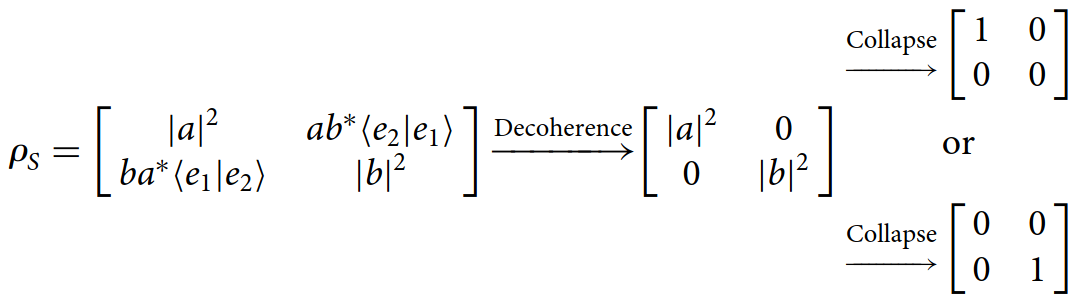
\includegraphics[width=\textwidth]{Images/Collapse_Measurement.png}
    \caption{Representasi konseptual hubungan antara dekoherensi dan keruntuhan keadaan kuantum. Interaksi sistem dengan lingkungan menyebabkan hilangnya elemen koherensi (\textit{off-diagonaal}) pada matriks densitas, sedangkan proses pengukuran memproyeksikan sistem ke salah satu keadaan eigen yang terdefinisi.}
    \label{fig:collapse_measurement}
\end{figure}